\documentclass[a4paper,10pt]{report}
\usepackage[utf8]{inputenc}
\usepackage[T1]{fontenc}
\usepackage[french]{babel}
\usepackage{lmodern} %pack de police
\usepackage{makeidx}
\usepackage{graphicx}
\usepackage{tikz}
\usepackage{eurosym}
\usepackage{colortbl}
\usepackage[table]{xcolor}
\usepackage{enumerate}
\usepackage[left=2cm, right=2cm, top=2cm, bottom=2cm]{geometry}
\usepackage{xcolor,listings}
\usepackage{textcomp}
\lstset{upquote=true}



\title{\textbf{Rapport Mini-Projet}Base de Données Objet Relationnelle}
\author{Tamara \bsc{Rocacher}~~-~~Meryll \bsc{Essig}}
\date{\today}
\makeindex


\makeatletter
\newcommand{\lstuppercase}{\uppercase\expandafter{\expandafter\lst@token
                           \expandafter{\the\lst@token}}}
\newcommand{\lstlowercase}{\lowercase\expandafter{\expandafter\lst@token
                           \expandafter{\the\lst@token}}}
\makeatother
\definecolor{blue}{rgb}{0.0,0.0,0.6}
\definecolor{green}{rgb}{0.0,0.6,0.0}
\definecolor{pink}{rgb}{0.6,0.0,0.6}
\definecolor{forestgreen}{RGB}{34,139,34}
\lstdefinestyle{Oracle}{basicstyle=\ttfamily,
                        breaklines=true,
                        keywordstyle=\lstuppercase,
                        emph={INSERT, INTO, VALUES, BEGIN, REPLACE, END,
                                      NEXTVAL, TO_NUMBER, TRUNC, LOAD, TRIGGER, FROM , TYPE, OR, CREATE, ON, BEFORE, AFTER, SEQUENCE, START, WITH, FOR, EACH, ROW, TABLE, AS, OBJECT},
                        emphstyle=\color{blue}\lstuppercase,
                        morecomment=[s][\color{forestgreen}]{"}{"},
                        numbers=left,
                        tag={0, 1, 2, 3, 4, 5, 6, 7, 8, 9},
                        tagstyle=\color{pink},
                        showstringspaces=false,
                        }
\lstdefinelanguage[Oracle]{SQL}[]{SQL}{
  morekeywords={INSERT, INTO, VALUES, BEGIN, REPLACE, END,
                NEXTVAL, TO_NUMBER, TRUNC, LOAD, TRIGGER, FROM , TYPE, OR, CREATE, ON, BEFORE, AFTER, SEQUENCE, START, WITH, FOR, EACH, ROW, TABLE, AS, OBJECT},
}
\lstset{language=[Oracle]SQL,
        style=Oracle
       }

\begin{document}
  \begin{titlepage}
  	\centering

{\scshape\LARGE Université de Montpellier \par}
  	\vspace{1cm}
{\scshape\Large Rapport du Mini-Projet Bases de Données Avancées\par}
  	\vspace{1.5cm}
    \vfill
  	{\huge\bfseries Base de Données Objet Relationnelle\par}
  	\vspace{2cm}


  	{\Large\itshape Tamara Rocacher~~-~~Meryll Essig\par}
  	\vspace{2cm}
  \vfill

  % Bottom of the page
 Ce rapport contient tout les scripts de création, remplissage et traitements demandés.

  \end{titlepage}


\tableofcontents


%Le contenu
\chapter{Introduction} % +/- 1 page
\section{Base de données}
  Une base de données Objet Relationnelle permet de stocker des informations et comportements associés à un objet de la vie réelle, en les regroupant dans un Type.
  Un Type correspond à une classe, mais les objets seront stockés de manière persistante, c'est à dire qu'ils ne seront pas éffacés après la fin de l'éxecution.
  L'aspect relationnel, quand à lui, permet de créer des liens entre ces objets (tables-type) ou avec d'autres tables, "simples".
\section{League of Legends}
  League of Legends est un jeu vidéo pour PC très complet au niveau des fonctionnalités. Un \textit{Joueur} y joue avec des \textit{Champions}, qui ont quatre \textit{capacités} propres à chacun d'eux. Les \textit{capacités} impactent le champion "émetteur" et/ou les autres champions en jeu, selon différents \textit{caractéristiques} (armure, dégats, vitesse d'attaque,...). Le \textit{Joueur} peut renforcer les \textit{Champions} en leur associant des pages de  \textit{Runes} et des \textit{Maîtrises}, qui permettent d'améliorer certaines \textit{caractéristiques} des \textit{Champions}. D'autre part, tout au long de la partie les \textit{caractéristiques} du \textit{Champion} pourront encore être améliorées avec des \textit{Items} (pour ne pas confondre Objets du jeux et Objets de la BD).
  Le choix des \textit{caractéristiques} à améliorer dépend des autres \textit{Champions} en jeux et de leurs \textit{caractéristiques} les plus renforcés. Le \textit{Joueur} doit donc avoir accès à tout ces renseignements pour prendre ces décisions, avant et pendant la partie.
\section{Approche}
  Au regard de la multitude d'objets présents dans le jeu, nous avons choisit l'approche OR. En effet, chaque champion en jeu est une instance d'un objet précis; décrit par ses critères et comportements associés. Chaque Item est aussi un objet, agissant possiblement sur tout les autres en jeu. D'autre part, dans le cadre d'un jeu video multijoueurs, les données les moins importantes, d'un point de vue Base de Données, sont implémentées dans l'algorithme.  L'approche OR nous permettra ainsi d'implementer un maximum de détails des comportements de chaque objet, au moyen des types et de plusieurs tables-objets.


\chapter{Conception}
Pour la suite, nous avons considéré que les caractéristiques des champions et les objets existants dans le jeu qui permettent  de les modifier, sont directement implémentés dans l'algorithme  du jeu. En effet, les champions, runes, items, etc, sont définis par des caractéristiques qui ne varient que rarement ( mise à jour par les développeurs du jeu) et il en existe un nombre limité (133 champions, 243 items, 297 runes et 45 maitrises à ce jour), au gré des ajouts des developpeurs. Ces données peuvent être stockées dans des fichiers externes, en JSON par exemple. Nous choisissons donc de ne stocker que les données reposant sur de nombreuses opérations "CRUD", représentant les objets possédés par le joueur, en tant que référence (appel) aux valeurs contenues dans les fichiers externes.

\section{Modèle conceptuel}
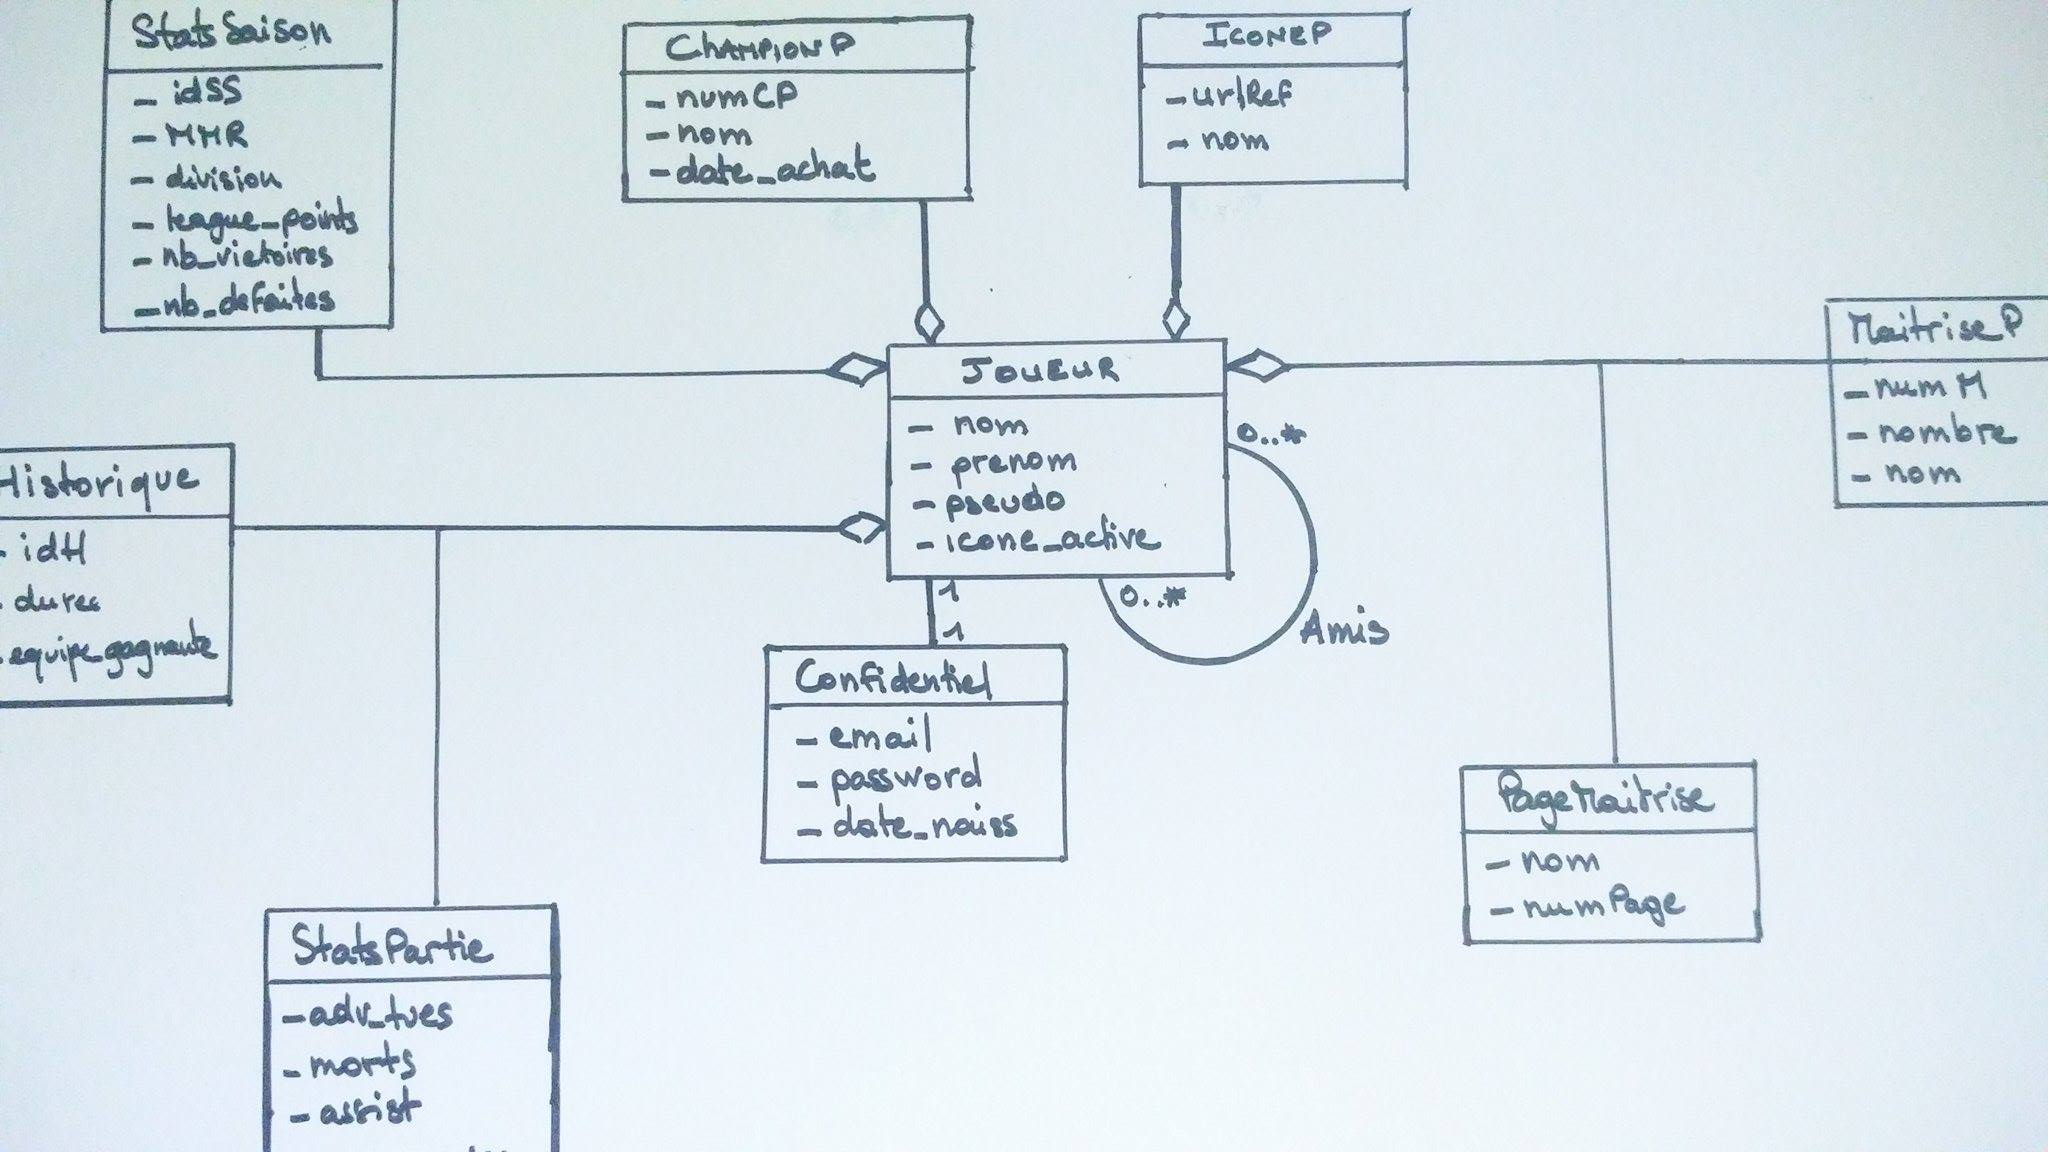
\includegraphics[scale=0.2]{uml.jpg}
\newpage
\section{Modèle logique}
\begin{lstlisting}

  Types: Confidentiel_t, Joueur_t, PageMaitrise_t, MaitriseP_t, Historique_t, IconeP_t, StatsPartie_t, StatsSaison_t, ChampionP_t, Ami_t

  Tables objets:
    Joueur(pseudo String,info_personnelles Confidentiel_t, icone_act String)
    Historique(idH Entier, duree_sec Entier, equipe_gagnante Entier)
    StatsPartie(joueur REF Joueur_t, Historique REF Historique_t, adv_tues Entier, morts Entier, assist Entier, num_equipe Entier)
    StatSaison( MMR Entier, division String, league_points Entier, nb_victoires Entier, nb_defaites Entier, joueur REF Joueur_t)
    ChampionsP(numCP Entier, joueur REF Joueur_t, date_achat Date)
    MaitriseP(numM Entier, nombre Entier, PageMaitrise PageMaitrise_t, joueur REF Joueur_t)
    IconeP(nom String, urlref String, joueur REF Joueur_t)
    Ami(joueur1 REF Joueur_t, joueur2 REF Joueur_t)

\end{lstlisting}


\chapter{Réalisation}
\section{Création}
D'apres l'approche que nous avons choisit, tout est Type:
\begin{lstlisting}
/*Creation des types*/


CREATE OR REPLACE TYPE Confidentiel_t AS OBJECT (email VARCHAR(50), password VARCHAR(255), nom VARCHAR(20), prenom VARCHAR(20), date_naissance DATE);
/
CREATE OR REPLACE TYPE Joueur_t AS OBJECT (pseudo VARCHAR(50), info_personnelles Confidentiel_t, icone_act VARCHAR(50));
/
CREATE OR REPLACE TYPE PageMaitrise_t AS OBJECT (nom VARCHAR(50), num_page NUMBER(2));
/
CREATE OR REPLACE TYPE Historique_t AS OBJECT (idH NUMBER(7), duree_sec NUMBER(5), equipe_gagnante NUMBER(1));
/
CREATE OR REPLACE TYPE IconeP_t AS OBJECT (urlref VARCHAR(255), nom VARCHAR(50), joueur REF Joueur_t);
/
CREATE OR REPLACE TYPE StatsPartie_t AS OBJECT (joueur REF Joueur_t, historique REF Historique_t, championJoue VARCHAR(20), adv_tues NUMBER(3), morts NUMBER(3), assist NUMBER(3), num_equipe NUMBER(1));
/
CREATE OR REPLACE TYPE StatsSaison_t AS OBJECT (MMR NUMBER(5), division VARCHAR(30), league_points NUMBER(3), nb_victoires NUMBER(5), nb_defaites NUMBER(5), joueur REF Joueur_t);
/
CREATE OR REPLACE TYPE ChampionP_t AS OBJECT (numCP NUMBER(7), joueur REF Joueur_t, date_achat DATE);
/
CREATE OR REPLACE TYPE MaitriseP_t AS OBJECT (joueur REF Joueur_t, pMaitrise PageMaitrise_t, numM NUMBER(7), nombre NUMBER(1));
/
CREATE OR REPLACE TYPE Ami_t AS OBJECT (joueur1 REF Joueur_t, joueur2 REF Joueur_t);
/
\end{lstlisting}

Les tables-objets sont données par les Types principaux:
\begin{lstlisting}

/*Creation des tables objet*/
CREATE TABLE MaitriseP OF MaitriseP_t;
CREATE TABLE IconeP OF IconeP_t;
CREATE TABLE Joueur OF Joueur_t(CONSTRAINT ps_pk PRIMARY KEY(pseudo));
CREATE TABLE StatsPartie OF StatsPartie_t;
CREATE TABLE ChampionP OF ChampionP_t;
CREATE TABLE StatsSaison OF StatsSaison_t;
CREATE TABLE Historique OF Historique_t(CONSTRAINT idh_pk PRIMARY KEY(idH));
CREATE TABLE Ami OF Ami_t;


/*Trigger permettant l'auto-incrementation*/
CREATE SEQUENCE historique_seq START WITH 1;

CREATE OR REPLACE TRIGGER historique_bir
BEFORE INSERT ON Historique
FOR EACH ROW

BEGIN
  SELECT historique_seq.NEXTVAL
  INTO   :new.idH
  FROM   dual;
END;
/

\end{lstlisting}



\section{Remplissage}
Nous avons peuplé la Base de données avec différents Joueurs, des parties dans l'Historique, des Maitrises, Champions et Amis.
Voir Annexes pour le détail (p 10).



\section{Traitements}
Voici des exemples de requêtes pour l'utilisation de la Base de Données:
\begin{lstlisting}

  /* Partie la plus courte jouée par le joueur 'clement' */
  SELECT h.idH, h.duree_sec  FROM Historique h WHERE h.duree_sec <= (SELECT MIN(s.historique.duree_sec) FROM Joueur j, StatsPartie s WHERE s.joueur=REF(j) AND j.pseudo='clement') AND ROWNUM <= 1;

  /* Liste des amis de clement */
  SELECT a.joueur2.pseudo FROM Ami a WHERE a.joueur1.pseudo='clement'
  UNION ALL
  SELECT a.joueur1.pseudo FROM Ami a WHERE a.joueur2.pseudo='clement';

  /* joueur possédant le plus de champions */
  SELECT j.pseudo FROM Joueur j, ChampionP c WHERE c.joueur=REF(j) HAVING COUNT(*) >= ALL (SELECT COUNT(*) FROM ChampionP c2 GROUP BY c2.joueur) GROUP BY j.pseudo;

  /* Joueur ayant le plus gros ratio Victoire/Defaites pour la saison */
  SELECT j.pseudo FROM Joueur j, StatsSaison s WHERE s.joueur=REF(j) AND (s.nb_victoires/s.nb_defaites) >= ALL (SELECT (s2.nb_victoires/s2.nb_defaites) FROM StatsSaison s2);

  /* Update des maitrises: ajout de 2 maitrises num 112*/
  UPDATE MaitriseP M SET M.nombre = M.nombre +2 WHERE M.numM = 112;
  SELECT m.nombre FROM MaitriseP m WHERE m.numM = 112; /*verification update */

  /* Joueur avec le plus de maitrises */
  SELECT j.pseudo FROM Joueur j, MaitriseP m WHERE REF(j) = m.joueur  HAVING COUNT(*) >= ALL (SELECT COUNT(*) FROM MaitriseP m2 GROUP BY m2.joueur) GROUP BY j.pseudo;

  /* Champion le plus joué (lux d'après les insertions) */
  SELECT st.championJoue, COUNT(*) FROM StatsPartie st  HAVING COUNT(*) >= ALL(SELECT COUNT(*) FROM StatsPartie st2 GROUP BY st2.championJoue) GROUP BY st.championJoue;

  /* Partie la plus longue de tous les temps */
  SELECT h.idH FROM Historique h WHERE duree_sec >= ALL ( SELECT h2.duree_sec FROM Historique h2);
  SELECT h.idH , h.duree_sec FROM  Historique h ;

  /* Statistiques de la dernièr partie jouée du joueur le mieux classé de la saison */
  SELECT championJoue, adv_tues, morts, assist, sp.joueur.pseudo  FROM StatsPartie sp, StatsSaison ss WHERE sp.joueur = ss.joueur AND sp.historique.idH >= ALL (SELECT h2.idH FROM Historique h2) AND ss.MMR >= ALL (SELECT sts.MMR FROM StatsSaison sts ) ;

  /* Joueur avec le meilleur ratio (kill + assists / death) de la partie la plus récente (idH max)*/
  SELECT  sp.joueur.pseudo , ((sp.adv_tues +sp.assist)/sp.morts)  FROM StatsPartie sp, Historique h WHERE REF(h) = sp.historique AND h.idH >= ALL (SELECT h2.idH FROM Historique h2) AND ((sp.adv_tues +sp.assist)/sp.morts)  >= ALL (SELECT ((sp2.adv_tues+ sp2.assist)/sp2.morts) FROM StatsPartie sp2 );


  /*Recherche d'un joueur par son pseudo pour pouvoir ajouter des amis*/
  SELECT j.pseudo FROM Joueur j WHERE  REGEXP_LIKE (j.pseudo,'*Dragon*' );


\end{lstlisting}




\chapter{Annexes} % Conclusions 1/2
\section{Suppression de la base}
Nous avons utilisé un script qui permet de supprimer toutes les tables en une seule fois. Cependant, a cause d'inter-dépendances, il faut le relancer 3 fois:
\begin{lstlisting}

  /* Script pour supprimer toutes les entrees de la base*/
  BEGIN
     FOR cur_rec IN (SELECT object_name, object_type
                       FROM user_objects
                      WHERE object_type IN
                               ('TABLE',
                                'VIEW',
                                'PACKAGE',
                                'PROCEDURE',
                                'FUNCTION',
                                'SEQUENCE',
                                'TYPE'
                               ))
     LOOP
        BEGIN
           IF cur_rec.object_type = 'TABLE'
           THEN
              EXECUTE IMMEDIATE    'DROP '
                                || cur_rec.object_type
                                || ' "'
                                || cur_rec.object_name
                                || '" CASCADE CONSTRAINTS';
           ELSE
              EXECUTE IMMEDIATE    'DROP '
                                || cur_rec.object_type
                                || ' "'
                                || cur_rec.object_name
                                || '"';
           END IF;
        EXCEPTION
           WHEN OTHERS
           THEN
              DBMS_OUTPUT.put_line (   'FAILED: DROP '
                                    || cur_rec.object_type
                                    || ' "'
                                    || cur_rec.object_name
                                    || '"'
                                   );
        END;
     END LOOP;
  END;
  /
\end{lstlisting}
\section{Remplissage}
Nous avons rempli la base de données comme suit:
\begin{lstlisting}


    /*Remplissage de la base de données*/
    INSERT INTO Joueur VALUES ('Exece', Confidentiel_t('jean.bon@mail.com', 'zzzgaze', 'Bon', 'Jean', TO_DATE('11-11-1991', 'DD-MM-YYYY')), 'Duck');
    INSERT INTO Joueur VALUES ('Michou', Confidentiel_t('michou@mail.com', 'z5415', 'Rosty', 'Michel', TO_DATE('10-11-1981', 'DD-MM-YYYY')), 'Duck');
    INSERT INTO Joueur VALUES ('blabla', Confidentiel_t('blabla@mail.com', 'z5415', 'bla', 'bla', TO_DATE('11-11-1991', 'DD-MM-YYYY')), 'FlappyBird');
    INSERT INTO Joueur VALUES ('xXDragonForceXx', Confidentiel_t('dragon@mail.com', 'z5415', 'Dragon', 'Nogard', TO_DATE('11-11-1991', 'DD-MM-YYYY')), 'Duck');
    INSERT INTO Joueur VALUES ('FlamerDu93', Confidentiel_t('flame@mail.com', 'z5415', 'Flame', 'Falme', TO_DATE('11-11-1991', 'DD-MM-YYYY')), 'Fish');
    INSERT INTO Joueur VALUES ('Cortex91LesPyramides', ConfidentielSELECT championJoue, adv_tues, morts, assist, sp.joueur.pseudo  FROM StatsPartie sp, StatsSaison ss WHERE sp.joueur = ss.joueur AND sp.historique.idH >= ALL (SELECT h2.idH FROM Historique h2) AND ss.MMR >= ALL (SELECT sts.MMR FROM StatsSaison sts ) ;_t('cortex@mail.com', 'z5415', 'Cortex', '91CdlaPatateMonFrer', TO_DATE('11-11-1991', 'DD-MM-YYYY')), 'Fish');
    INSERT INTO Joueur VALUES ('flo', Confidentiel_t('flo@mail.com', 'z5415', 'Flo', 'olf', TO_DATE('11-11-1991', 'DD-MM-YYYY')), 'Hur');
    INSERT INTO Joueur VALUES ('clement', Confidentiel_t('@mail.com', 'z5415', 'Clement', 'Chelmi', TO_DATE('11-11-1991', 'DD-MM-YYYY')), 'Duck');
    INSERT INTO Joueur VALUES ('coucou', Confidentiel_t('@mail.com', 'z5415', 'Cou', 'Cou', TO_DATE('11-11-1991', 'DD-MM-YYYY')), 'Hur');
    INSERT INTO Joueur VALUES ('ILikeTrains', Confidentiel_t('iliketrains@mail.com', 'z5415', 'iLike', 'Trains', TO_DATE('11-11-1991', 'DD-MM-YYYY')), 'Fish');
    INSERT INTO Joueur VALUES ('Morsay', Confidentiel_t('truand2lagalere@mail.com', 'z5415', 'Morsay', '', TO_DATE('11-11-1991', 'DD-MM-YYYY')), 'FlappyBird');

    INSERT INTO StatsSaison VALUES (StatsSaison_t(3000, 'Platine 5', 100, 800, 600, (SELECT REF(j) FROM Joueur j WHERE j.pseudo='Exece')));
    INSERT INTO StatsSaison VALUES (StatsSaison_t(2464, 'Argent 4', 20, 30, 60, (SELECT REF(j) FROM Joueur j WHERE j.pseudo='Michou')));
    INSERT INTO StatsSaison VALUES (StatsSaison_t(2948, 'Or 2', 20, 30, 40, (SELECT REF(j) FROM Joueur j WHERE j.pseudo='blabla')));
    INSERT INTO StatsSaison VALUES (StatsSaison_t(5000, 'Diamant 2', 30, 200, 70, (SELECT REF(j) FROM Joueur j WHERE j.pseudo='xXDragonForceXx')));
    INSERT INTO StatsSaison VALUES (StatsSaison_t(2051, 'Bronze 1', 10, 30, 10, (SELECT REF(j) FROM Joueur j WHERE j.pseudo='FlamerDu93')));
    INSERT INTO StatsSaison VALUES (StatsSaison_t(2047, 'Bronze 1', 20, 280, 600, (SELECT REF(j) FROM Joueur j WHERE j.pseudo='Cortex91LesPyramides')));
    INSERT INTO StatsSaison VALUES (StatsSaison_t(2353, 'Argent 5', 80, 50, 60, (SELECT REF(j) FROM Joueur j WHERE j.pseudo='flo')));
    INSERT INTO StatsSaison VALUES (StatsSaison_t(2051, 'Bronze 3', 20, 30, 90, (SELECT REF(j) FROM Joueur j WHERE j.pseudo='clement')));
    INSERT INTO StatsSaison VALUES (StatsSaison_t(2371, 'Argent 4', 20, 130, 110, (SELECT REF(j) FROM Joueur j WHERE j.pseudo='coucou')));
    INSERT INTO StatsSaison VALUES (StatsSaison_t(2851, 'Or 5', 50, 500, 60, (SELECT REF(j) FROM Joueur j WHERE j.pseudo='ILikeTrains')));
    INSERT INTO StatsSaison VALUES (StatsSaison_t(2052, 'Bronze 5', 20, 300, 1000, (SELECT REF(j) FROM Joueur j WHERE j.pseudo='Morsay')));


    INSERT INTO IconeP VALUES ('https://dfdf.com', 'Duck', (SELECT REF(j) FROM Joueur j WHERE j.pseudo='Morsay'));
    INSERT INTO IconeP VALUES ('https://dfdf.com', 'FlappyBird', (SELECT REF(j) FROM Joueur j WHERE j.pseudo='Morsay'));
    INSERT INTO IconeP VALUES ('https://dfdf.com', 'Duck', (SELECT REF(j) FROM Joueur j WHERE j.pseudo='xXDragonForceXx'));
    INSERT INTO IconeP VALUES ('https://dfdf.com', 'FlappyBird', (SELECT REF(j) FROM Joueur j WHERE j.pseudo='xXDragonForceXx'));
    INSERT INTO IconeP VALUES ('https://dfdf.com', 'Harambe', (SELECT REF(j) FROM Joueur j WHERE j.pseudo='xXDragonForceXx'));
    INSERT INTO IconeP VALUES ('https://dfdf.com', 'Fish', (SELECT REF(j) FROM Joueur j WHERE j.pseudo='FlamerDu93'));
    INSERT INTO IconeP VALUES ('https://dfdf.com', 'Duck', (SELECT REF(j) FROM Joueur j WHERE j.pseudo='Cortex91LesPyramides'));


    INSERT INTO MaitriseP VALUES (MaitriseP_t((SELECT REF(j) FROM Joueur j WHERE j.pseudo='ILikeTrains'), PageMaitrise_t('ADC Std', 1), 42, 5));
    INSERT INTO MaitriseP VALUES (MaitriseP_t((SELECT REF(j) FROM Joueur j WHERE j.pseudo='ILikeTrains'), PageMaitrise_t('ADC Std', 1), 15, 5));
    INSERT INTO MaitriseP VALUES (MaitriseP_t((SELECT REF(j) FROM Joueur j WHERE j.pseudo='ILikeTrains'), PageMaitrise_t('ADC Std', 1), 10, 5));
    INSERT INTO MaitriseP VALUES (MaitriseP_t((SELECT REF(j) FROM Joueur j WHERE j.pseudo='ILikeTrains'), PageMaitrise_t('ADC Std', 1), 68, 5));
    INSERT INTO MaitriseP VALUES (MaitriseP_t((SELECT REF(j) FROM Joueur j WHERE j.pseudo='ILikeTrains'), PageMaitrise_t('ADC Std', 1), 230, 5));
    INSERT INTO MaitriseP VALUES (MaitriseP_t((SELECT REF(j) FROM Joueur j WHERE j.pseudo='ILikeTrains'), PageMaitrise_t('ADC Std', 1), 3, 5));
    INSERT INTO MaitriseP VALUES (MaitriseP_t((SELECT REF(j) FROM Joueur j WHERE j.pseudo='xXDragonForceXx'), PageMaitrise_t('Mage Std', 1), 42, 5));
    INSERT INTO MaitriseP VALUES (MaitriseP_t((SELECT REF(j) FROM Joueur j WHERE j.pseudo='xXDragonForceXx'), PageMaitrise_t('Mage Std', 1), 51, 5));
    INSERT INTO MaitriseP VALUES (MaitriseP_t((SELECT REF(j) FROM Joueur j WHERE j.pseudo='xXDragonForceXx'), PageMaitrise_t('Mage Std', 1), 112, 5));
    INSERT INTO MaitriseP VALUES (MaitriseP_t((SELECT REF(j) FROM Joueur j WHERE j.pseudo='xXDragonForceXx'), PageMaitrise_t('Mage Std', 1), 242, 5));
    INSERT INTO MaitriseP VALUES (MaitriseP_t((SELECT REF(j) FROM Joueur j WHERE j.pseudo='xXDragonForceXx'), PageMaitrise_t('Mage Std', 1), 182, 5));
    INSERT INTO MaitriseP VALUES (MaitriseP_t((SELECT REF(j) FROM Joueur j WHERE j.pseudo='xXDragonForceXx'), PageMaitrise_t('Mage Std', 1), 1, 1));
    INSERT INTO MaitriseP VALUES (MaitriseP_t((SELECT REF(j) FROM Joueur j WHERE j.pseudo='xXDragonForceXx'), PageMaitrise_t('Mage Std', 1), 3, 5));
    INSERT INTO MaitriseP VALUES (MaitriseP_t((SELECT REF(j) FROM Joueur j WHERE j.pseudo='xXDragonForceXx'), PageMaitrise_t('Mage Std', 1), 87, 5));
    INSERT INTO MaitriseP VALUES (MaitriseP_t((SELECT REF(j) FROM Joueur j WHERE j.pseudo='xXDragonForceXx'), PageMaitrise_t('Mage Std', 1), 69, 5));
    INSERT INTO MaitriseP VALUES (MaitriseP_t((SELECT REF(j) FROM Joueur j WHERE j.pseudo='xXDragonForceXx'), PageMaitrise_t('Mage Std', 1), 75, 5));
    INSERT INTO MaitriseP VALUES (MaitriseP_t((SELECT REF(j) FROM Joueur j WHERE j.pseudo='xXDragonForceXx'), PageMaitrise_t('Mage Std', 1), 17, 5));


    INSERT INTO ChampionP VALUES (1, (SELECT REF(j) FROM Joueur j WHERE j.pseudo='FlamerDu93'), TO_DATE('21-12-2012', 'DD-MM-YYYY'));
    INSERT INTO ChampionP VALUES (2, (SELECT REF(j) FROM Joueur j WHERE j.pseudo='FlamerDu93'), TO_DATE('21-12-2012', 'DD-MM-YYYY'));
    INSERT INTO ChampionP VALUES (3, (SELECT REF(j) FROM Joueur j WHERE j.pseudo='FlamerDu93'), TO_DATE('21-12-2012', 'DD-MM-YYYY'));
    INSERT INTO ChampionP VALUES (4, (SELECT REF(j) FROM Joueur j WHERE j.pseudo='xXDragonForceXx'), TO_DATE('21-12-2012', 'DD-MM-YYYY'));
    INSERT INTO ChampionP VALUES (5, (SELECT REF(j) FROM Joueur j WHERE j.pseudo='FlamerDu93'), TO_DATE('21-12-2012', 'DD-MM-YYYY'));
    INSERT INTO ChampionP VALUES (1, (SELECT REF(j) FROM Joueur j WHERE j.pseudo='xXDragonForceXx'), TO_DATE('21-12-2012', 'DD-MM-YYYY'));
    INSERT INTO ChampionP VALUES (25, (SELECT REF(j) FROM Joueur j WHERE j.pseudo='xXDragonForceXx'), TO_DATE('21-12-2012', 'DD-MM-YYYY'));
    INSERT INTO ChampionP VALUES (89, (SELECT REF(j) FROM Joueur j WHERE j.pseudo='FlamerDu93'), TO_DATE('21-12-2012', 'DD-MM-YYYY'));
    INSERT INTO ChampionP VALUES (64, (SELECT REF(j) FROM Joueur j WHERE j.pseudo='xXDragonForceXx'), TO_DATE('21-12-2012', 'DD-MM-YYYY'));
    INSERT INTO ChampionP VALUES (118, (SELECT REF(j) FROM Joueur j WHERE j.pseudo='ILikeTrains'), TO_DATE('21-12-2012', 'DD-MM-YYYY'));





    INSERT INTO Ami VALUES ((SELECT REF(j) FROM Joueur j WHERE j.pseudo='Exece'),(SELECT REF(j) FROM Joueur j WHERE j.pseudo='Michou'));
    INSERT INTO Ami VALUES ((SELECT REF(j) FROM Joueur j WHERE j.pseudo='Exece'),(SELECT REF(j) FROM Joueur j WHERE j.pseudo='ILikeTrains'));
    INSERT INTO Ami VALUES ((SELECT REF(j) FROM Joueur j WHERE j.pseudo='Exece'),(SELECT REF(j) FROM Joueur j WHERE j.pseudo='clement'));
    INSERT INTO Ami VALUES ((SELECT REF(j) FROM Joueur j WHERE j.pseudo='blabla'),(SELECT REF(j) FROM Joueur j WHERE j.pseudo='clement'));
    INSERT INTO Ami VALUES ((SELECT REF(j) FROM Joueur j WHERE j.pseudo='clement'),(SELECT REF(j) FROM Joueur j WHERE j.pseudo='flo'));
    INSERT INTO Ami VALUES ((SELECT REF(j) FROM Joueur j WHERE j.pseudo='clement'),(SELECT REF(j) FROM Joueur j WHERE j.pseudo='xXDragonForceXx'));



    /*Les parties sont liees à 10 joueurs differents, et doivent etre inserées conjointement*/
    DECLARE
    idHist number;
    BEGIN
      INSERT INTO Historique (duree_sec, equipe_gagnante) VALUES (3100, 2);
      SELECT MAX(idH) INTO idHist FROM Historique;
      INSERT INTO StatsPartie VALUES(StatsPartie_t((SELECT REF(j) FROM Joueur j WHERE j.pseudo='Exece'), (SELECT REF(h) FROM Historique h WHERE idH=idHist), 'Katarina', 2, 9, 14, 2));
      INSERT INTO StatsPartie VALUES(StatsPartie_t((SELECT REF(j) FROM Joueur j WHERE j.pseudo='Michou'), (SELECT REF(h) FROM Historique h WHERE idH=idHist), 'RekSai', 10, 9, 14, 2));
      INSERT INTO StatsPartie VALUES(StatsPartie_t((SELECT REF(j) FROM Joueur j WHERE j.pseudo='FlamerDu93'), (SELECT REF(h) FROM Historique h WHERE idH=idHist), 'Jhin', 2, 9, 14, 2));
      INSERT INTO StatsPartie VALUES(StatsPartie_t((SELECT REF(j) FROM Joueur j WHERE j.pseudo='flo'), (SELECT REF(h) FROM Historique h WHERE idH=idHist), 'Ezreal', 2, 9, 14, 2));
      INSERT INTO StatsPartie VALUES(StatsPartie_t((SELECT REF(j) FROM Joueur j WHERE j.pseudo='coucou'), (SELECT REF(h) FROM Historique h WHERE idH=idHist), 'Khazix', 2, 9, 14, 2));
      INSERT INTO StatsPartie VALUES(StatsPartie_t((SELECT REF(j) FROM Joueur j WHERE j.pseudo='Cortex91LesPyramides'), (SELECT REF(h) FROM Historique h WHERE idH=idHist), 'Lulu', 1, 3, 14, 1));
      INSERT INTO StatsPartie VALUES(StatsPartie_t((SELECT REF(j) FROM Joueur j WHERE j.pseudo='ILikeTrains'), (SELECT REF(h) FROM Historique h WHERE idH=idHist), 'Bard', 2, 9, 14, 1));
      INSERT INTO StatsPartie VALUES(StatsPartie_t((SELECT REF(j) FROM Joueur j WHERE j.pseudo='Morsay'), (SELECT REF(h) FROM Historique h WHERE idH=idHist), 'Nocturne', 2, 9, 14, 1));
      INSERT INTO StatsPartie VALUES(StatsPartie_t((SELECT REF(j) FROM Joueur j WHERE j.pseudo='xXDragonForceXx'), (SELECT REF(h) FROM Historique h WHERE idH=idHist), 'Zed', 31, 5, 1, 1));
      INSERT INTO StatsPartie VALUES(StatsPartie_t((SELECT REF(j) FROM Joueur j WHERE j.pseudo='clement'), (SELECT REF(h) FROM Historique h WHERE idH=idHist), 'Lux', 2, 9, 14, 1));
    END;
    /

    DECLARE
    idHist number;
    BEGIN
      INSERT INTO Historique (duree_sec, equipe_gagnante) VALUES (1200, 2);
      SELECT MAX(idH) INTO idHist FROM Historique;
      INSERT INTO StatsPartie VALUES(StatsPartie_t((SELECT REF(j) FROM Joueur j WHERE j.pseudo='blabla'), (SELECT REF(h) FROM Historique h WHERE idH=idHist), 'Katarina', 2, 9, 14, 2));
      INSERT INTO StatsPartie VALUES(StatsPartie_t((SELECT REF(j) FROM Joueur j WHERE j.pseudo='Michou'), (SELECT REF(h) FROM Historique h WHERE idH=idHist), 'RekSai', 10, 9, 14, 2));
      INSERT INTO StatsPartie VALUES(StatsPartie_t((SELECT REF(j) FROM Joueur j WHERE j.pseudo='FlamerDu93'), (SELECT REF(h) FROM Historique h WHERE idH=idHist), 'Lux', 2, 9, 14, 2));
      INSERT INTO StatsPartie VALUES(StatsPartie_t((SELECT REF(j) FROM Joueur j WHERE j.pseudo='flo'), (SELECT REF(h) FROM Historique h WHERE idH=idHist), 'Ezreal', 2, 9, 14, 2));
      INSERT INTO StatsPartie VALUES(StatsPartie_t((SELECT REF(j) FROM Joueur j WHERE j.pseudo='coucou'), (SELECT REF(h) FROM Historique h WHERE idH=idHist), 'Khazix', 2, 9, 14, 2));
      INSERT INTO StatsPartie VALUES(StatsPartie_t((SELECT REF(j) FROM Joueur j WHERE j.pseudo='Cortex91LesPyramides'), (SELECT REF(h) FROM Historique h WHERE idH=idHist), 'Lulu', 1, 3, 14, 1));
      INSERT INTO StatsPartie VALUES(StatsPartie_t((SELECT REF(j) FROM Joueur j WHERE j.pseudo='ILikeTrains'), (SELECT REF(h) FROM Historique h WHERE idH=idHist), 'Bard', 2, 9, 14, 1));
      INSERT INTO StatsPartie VALUES(StatsPartie_t((SELECT REF(j) FROM Joueur j WHERE j.pseudo='Morsay'), (SELECT REF(h) FROM Historique h WHERE idH=idHist), 'Nocturne', 2, 9, 14, 1));
      INSERT INTO StatsPartie VALUES(StatsPartie_t((SELECT REF(j) FROM Joueur j WHERE j.pseudo='xXDragonForceXx'), (SELECT REF(h) FROM Historique h WHERE idH=idHist), 'Zed', 31, 5, 1, 1));
      INSERT INTO StatsPartie VALUES(StatsPartie_t((SELECT REF(j) FROM Joueur j WHERE j.pseudo='clement'), (SELECT REF(h) FROM Historique h WHERE idH=idHist), 'Lux', 2, 9, 14, 1));
    END;
    /

    DECLARE
    idHist number;
    BEGIN
      INSERT INTO Historique (duree_sec, equipe_gagnante) VALUES (1800, 2);
      SELECT MAX(idH) INTO idHist FROM Historique;
      INSERT INTO StatsPartie VALUES(StatsPartie_t((SELECT REF(j) FROM Joueur j WHERE j.pseudo='Michou'), (SELECT REF(h) FROM Historique h WHERE idH=idHist), 'Katarina', 2, 9, 14, 2));
      INSERT INTO StatsPartie VALUES(StatsPartie_t((SELECT REF(j) FROM Joueur j WHERE j.pseudo='Cortex91LesPyramides'), (SELECT REF(h) FROM Historique h WHERE idH=idHist), 'RekSai', 10, 9, 14, 2));
      INSERT INTO StatsPartie VALUES(StatsPartie_t((SELECT REF(j) FROM Joueur j WHERE j.pseudo='blabla'), (SELECT REF(h) FROM Historique h WHERE idH=idHist), 'Bard', 2, 9, 14, 2));
      INSERT INTO StatsPartie VALUES(StatsPartie_t((SELECT REF(j) FROM Joueur j WHERE j.pseudo='flo'), (SELECT REF(h) FROM Historique h WHERE idH=idHist), 'Ezreal', 2, 9, 14, 2));
      INSERT INTO StatsPartie VALUES(StatsPartie_t((SELECT REF(j) FROM Joueur j WHERE j.pseudo='coucou'), (SELECT REF(h) FROM Historique h WHERE idH=idHist), 'Khazix', 2, 9, 14, 2));
      INSERT INTO StatsPartie VALUES(StatsPartie_t((SELECT REF(j) FROM Joueur j WHERE j.pseudo='Morsay'), (SELECT REF(h) FROM Historique h WHERE idH=idHist), 'Lulu', 1, 3, 14, 1));
      INSERT INTO StatsPartie VALUES(StatsPartie_t((SELECT REF(j) FROM Joueur j WHERE j.pseudo='ILikeTrains'), (SELECT REF(h) FROM Historique h WHERE idH=idHist), 'Bard', 2, 9, 14, 1));
      INSERT INTO StatsPartie VALUES(StatsPartie_t((SELECT REF(j) FROM Joueur j WHERE j.pseudo='xXDragonForceXx'), (SELECT REF(h) FROM Historique h WHERE idH=idHist), 'Nocturne', 2, 9, 14, 1));
      INSERT INTO StatsPartie VALUES(StatsPartie_t((SELECT REF(j) FROM Joueur j WHERE j.pseudo='clement'), (SELECT REF(h) FROM Historique h WHERE idH=idHist), 'Miss Fortune', 31, 5, 1, 1));
      INSERT INTO StatsPartie VALUES(StatsPartie_t((SELECT REF(j) FROM Joueur j WHERE j.pseudo='FlamerDu93'), (SELECT REF(h) FROM Historique h WHERE idH=idHist), 'Lux', 2, 9, 14, 1));
    END;
    /

\end{lstlisting}
\end{document}
